\chapter{Supernova Remnants: Observation and Theory}\label{chap:Rems}

\section{Identification and Classification of Supernova Remnants}\label{Rems:intro}
When a massive star at the end stage of its evolution explodes as a supernova, it nearly instantaneously injects a massive amount of kinetic energy into the surrounding medium ($\sim 10^{51}$ erg). The supersonically expanding blast-wave, ejected stellar mass, and possible compact stellar remnant comprise an \snr{}. The first two identified \snrs{} (the Crab and Kepler's \snr{}) were initially observed as optical nebulosities found to be associated with historical supernovae (see Figure \ref{fig:Crab}). It was not until the advent of the radio interferometer that a number of these nebulae were discovered and could thus be studied as a population.  In fact, one of the first discrete radio objects to be detected was a remnant in the Cassiopeia constellation now known as Cassiopeia A \citep{Ryle48}.

\begin{figure*}[h!]
	\begin{center}
		%\hspace*{-1.5cm} 
		\begin{tabular}{ll}
			\includegraphics[width=0.5\columnwidth]{Figures/{rosseCrab1}.png} &
			\includegraphics[width=0.5\columnwidth]{Figures/{rosseCrab2}.jpg} \\
		\end{tabular}
	\end{center}
	\caption[Historical Crab nebula drawings]{
		\label{fig:Crab}{Left: First depiction of the Crab nebula by William Parsons, the Third Earl of Rosse,  based on his observations using a 36 inch telescope in 1844. The filamentary structure motivated him to dub it the Crab nebula. Right: Another depiction of the Crab nebula  by William Parson and R. J. Mitchell based on observations with a 72 inch telescope in 1884. From J. Bevis, Uranographia Britannica, 1750}
	}
\end{figure*}
One of the primary distinguishing features of the radio emission from \snrs{} was their distinctly non-thermal spectra (a \pl{} with flux  ${\rm S \propto \nu^\alpha}$, where $\nu$ is frequency). The clearly non-thermal emission was first proposed to arise from \sync{} radiation (and hence is emitted by a population of relativistic electrons) by \cite{Kiepenheuer50} and \cite{Alfven50}, and then by \cite{Shklovskii53} who correctly associated the remnants with supernovae in the Galaxy. To this day, \snrs{} are still primarily identified through radio observations (although a number have been first detected in X-ray as well). A catalog of 294 radio-identified Galactic \snrs{} is maintained at \url{http://www.mrao.cam.ac.uk/surveys/snrs/} by \cite{Green14} (referred to as Green's catalog) and a complementary high-energy catalog, summarizing the X-ray to \gam{} properties of Galactic \snr{}s, is upkept by \cite{Ferrand12} at \url{http://www.physics.umanitoba.ca/snr/SNRcat}

While the non-thermal, radio \sync{} spectra of  \snrs{} are used to identify remnants, their morphology is used to classify them. The classifications, based on radio and X-ray observations are:
\begin{itemize}
	\item \textbf{ Shell-type} \snrs{} are characterized by a radio (and sometimes X-ray) limb-brightened shell or ring. The perimeter or the (possibly incomplete) shell corresponds to the expanding forward shock from the blast-wave and is composed of the ejecta from the initial explosion as well as mass from the surrounding medium swept-up by the blast-wave. They are typically associated with less-evolved, or dynamically young \snrs{} (see the following Chapter for details on \snr{} evolution). In \cite{Green14}, 79\% of the radio \snrs{} are classified as shell type. 
	
	\item \textbf{Filled-center} \snrs{} or \textbf{plerions} are \snrs{} that show no clear shell structure but  rather are centrally bright at radio, and sometimes X-ray, energies. The central \sync{} emission arises if the  compact stellar remnant is a pulsar which can drive a \pwn{} \cite{Gaensler06}. The \pwn{} is generated by the rotational power of the spinning pulsar transferring its energy to a relativistic, magnetized wind of electrons and positrons that emit \sync{} radiation throughout the nebula. While the energy source of the shell-type \snr{} is deposited in the singular supernova event, the spin-down power of the pulsar is injected into the plerionic system over a much longer time span. 5\% of radio \snrs{} are center-filled \citep{Green14}.
	\item \textbf{Composite} remnants are simply \snrs{} that display both a  distinct shell-like structure as well as a center-filled, non-thermal \sync{} nebula.. \cite{Green14} classifies 12\% of \snrs{} as being composite.
	
	\item \textbf{Mixed morphology} \snrs{} are ones that exhibit a non-thermal radio shell-like structure as well as centrally located thermal X-ray emission \citep{Rho98}. This is in contrast to the composite system which displays a non-thermal emission nebula generated by a rotating neutron star. Some authors, including \cite{Green14}, use mixed-morphology interchangeably with composite. The thermal X-ray emission is produced by swept-up and shock-heated  material. These \snrs{} are often associated with more-evolved (or middle-aged) remnants that are interacting with surrounding, dense molecular material (as evidenced by shocked molecular lines and sometimes 1720 MHz OH masers). 
	\jamie{add kewl pic of each of the types shell:casA, tycho, kep, young! plerion: crab 3C58. comp: Vela?, mixed:IC443?}
\end{itemize}

The remaining few percent of \snrs{} not classified as one of the above are remnants that show a more complicated morphology, yet are still believed to be \snrs{}. In fact, with more sensitive, higher resolution telescopes, many shell-type \snrs{} only exhibit partially complete circular structures, and may show signs of blow-out (when part of the shell appears to expand faster in one direction than another) or elongated morphologies, all signs of not-purely spherical evolution of the blast-wave (which itself might not be spherically symmetric) in an inhomogeneous \ism{}.

\section{\label{Rems:evo}Supernova Remnant Dynamics and  Evolution}
The formation of an \snr{} begins as the supersonically traveling ejecta expands out and collides with the \ism{}  forming a blast-wave. The standard model for the evolution of an \snr{} (first proposed by \cite{Woltjer72}) is divided into four phases. 

\begin{enumerate}
	\item \textbf{ Free-Expansion Phase:} In this phase, (sometimes referred to as the ejecta-dominated phase), the forward shock of the blast-wave expands out into the \ism{} sweeping up mass as it expands. The ejecta mass is of the order of a few to 10's of \msun{}, while the shock speed is typically ${\rm \sim 10^3-10^4~ km~s^{-1}}$ for type Ia and core-collapse events respectively \cite{Reynolds08}. The velocity of the shock remains essentially constant in this phase until the mass of the swept-up material, equals that of the ejecta mass.
	At this point the swept-up mass starts to dynamically affect the expansion of the remnant, marking the end of the free-expansion phase.
	
	\item \textbf{\sedt{} Phase:} The \sedt{} phase (also referred to as the adiabatic expansion phase) begins when the swept-up mass ${\rm M_{su}}$, is equivalent to the ejecta mass, ${\rm M_{ej}}$. The radius of the \snr{} at the onset of the \sedt{} phase is given by:
	\begin{equation}
	R_{ST_0} = (3M_{ej}/4\pi \mu \rho_0)^{1/3} = 1.9(M_{ej}/n_0)^{1/3} pc,
	\end{equation}
	for ${\rm \rho_0 = n_0m_H}$, the mass density of the swept up matter, where 
	${\rm n_0}$ is the pre-shock particle density of the medium the \snr{} is expanding into (in units of ${\rm cm^{-3}}$), $\mu\approx1.4$ is the \ism{}'s mean atomic weight and ${\rm M_{ej}}$ is in units of \msun{}. The \sedt{} phase is dominated by the thermal pressure of the shock-heated gas which is adiabatically expanding (conserving energy), yet the gas is still hot enough that radiative losses are relatively inefficient. \cite{1959sdmm.book.....S} and \cite{Taylor50} developed a self-similar, analytic model for the evolution of the shock at this phase for an explosion that instantaneously injects energy at a point into a uniform density medium with no energy loss. The \sedt{} solution for the radius of a shock that evolves with time, t, for an explosion energy, E, is:
	\begin{equation}
	R_{ST} = \bigg{(}\zeta \frac{Et^2}{\rho_0} \bigg{)}^{{1/5}} = 0.314(E_{51}/n_0)^{1/5}t_{y}^{2/5} pc,
	\end{equation}
	with the constant, $\zeta = 2.026$ corresponding to a monatomic, non-relativistic  gas ($\gamma = 5/3$), E$_{51}$ the energy of the explosion in units of $10^{51}$ erg, and t given in years. This phase typically lasts for a few $10^4$ yr, with the radius of the \snr{} growing to 10's of pc. The \sedt{} phase ends when the temperature has decreased enough ($\approx 10^6 K$), through expansion and adiabatic cooling, that recombination can occur and atoms can cool radiatively.
	
	\item \textbf{Radiative Phase:} In the radiative phase, also known as the snowplow phase, the increased cooling causes the \snr{} shell to expand slower. Interior to the shock though, hot gas has not had time to cool and continues expanding adiabatically, exerting a pressure on the cooler, outer shell. The pressure of the hot interior pushes on the dense shell,  ``snowplowing'' ambient mass from the \ism{}, which will coast out, conserving momentum as the interior cools. 
	\item \textbf{Dispersion Phase:} Finally, the \snr{} diffuses and merges into the \ism{} with the temperature and shock velocity decreasing and becoming comparable to that of the ambient \ism{}.
\end{enumerate}

While this general scheme for the evolution of an \snr{} in the \ism{} is sufficient for explaining general observational features of \snrs{}, more intricate models are required to explain details of individual \snrs{}. Various authors have since expanded on the dynamical evolution of \snrs{} by including information regarding the initial velocity/density structure of the ejecta, inhomogeneities of the material the \snr{} is expanding into, energy loss through escaping \crs{}, and the effects of magnetic fields on expansion \citep[and references in \cite{Vink12} which reviews various analytic \snr{ expansion models}]{Chevalier74,Chevalier82,Truelove99}.
  
\section{\label{Rems:CR}The Supernova Remnant Cosmic Ray Connection}

As discussed in Chapter \ref{Rems:evo}, the massive amount of energy released by a supernova explosion goes into the creation of a blast-wave that expands out, shocking and heating the region around the progenitor star. It is thought that the cataclysmic explosion is the prime energy source and generator of Galactic \crs{} (at least up to the knee of the \cray{} energy spectrum, see Figure \ref{fig:CRspec}).  \crs{} are charged particles with energies ranging from about 1\mev{} to $10^{21}$ eV, first discovered, and shown to be of extra-terrestrial origin by \cite{Hess12}. \crs{} are a major source of energy in the \ism{} with an energy density,  ${\rm \rho_{CR} \sim 1~eV~cm^{-3}}$ \citep{Blasi13,Horandel08}. \crs{} account for about $1/3$ of the total energy density of the \ism{} and thus play a pivotal role in stoking chemical evolution and in  driving Galactic evolution. 

It was first proposed by \cite{Baade34} and then again, more quantitatively, by \cite{Ginzburg64} and \cite{Hayakawa69}, that supernovae could be the source of \crs{}. At the time, this was based solely on energy requirements since  there is a dearth of physical processes in the universe that can supply the appropriate energy to match the energy density in Galactic \crs{}. We can estimate the total power in \crs{} in the Galaxy as:

\begin{figure}[h!]%[t] 
	\centering
	\makebox[\linewidth]{\includegraphics[width=1.\columnwidth]{Figures/Blasi13_CRspec}}
	\caption[CR spectrum as measured at Earth]{\cray{} spectrum as measured at Earth. Protons are the dominant species accounting for  $\sim 99\%$ of the detected particles. The electron-to-proton ratio at 10\gev{} is  K$_{ep} \approx 0.01$. The so-called ``knee'' of the \cray{} energy spectrum occurs at $\sim 3\times 10^{15}$ eV, where the \pl{} spectral slope changes from $-2.7$ to $-3.1$. Above the knee, the \crs{} are believed to be of an extra-galactic origin. Figure from \cite{Blasi13}.
	\label{fig:CRspec}} 
\end{figure}

\begin{equation}\label{eq:crLum}
\rm {L_{CR} = \frac{V\rho_{CR}}{\tau} \sim 5\times 10^{40}~erg~s^{-1}}
\end{equation}
where the volume of the Galactic disk is, ${\rm V = \pi R^2 d \sim  \pi (15~kpc)^2(200~pc)}$ and ${\rm \tau \sim 6\times 10^6}$ yr is the residence time of \crs{} in the Galaxy determined from the boron to carbon ratio \citep{Gaisser90}. With the energy output of a single supernova event being $\sim 10^{51}$ erg, and a supernova rate in our Galaxy of $\sim$ 2-3 per century, supernovae supply a total power of about ${\rm 10^{42} erg~s^{-1}}$, and we see that the energy density of \crs{} in the Galaxy can be explained if about 10\% of the explosion energy goes into particle acceleration.

This energy argument is of course circumstantial, and a physical mechanism to explain the transfer of energy from explosion to shock, and shock to particles accelerated to very high energies is necessary. \cite{Fermi49} first proposed a mechanism by which charged particles can  gain energy by being magnetically ``reflected" back and forth by molecular clouds. In his initial formulation it seemed like it might not be a viable mechanism to explain \crs{} since the effects of reflection by receding and approaching clouds 
only produced energy gains in the second order terms of the ratio of cloud to particle velocity, resulting in slow acceleration rates. Several authors \citep[for example]{Bell78,Blandford78} noticed that in a strong shock there is a preferred frame (that of either the pre or post-shock scattering center) and particles crossing the shock will gain energy after every shock crossing as they are reflected multiple times by magnetic turbulence, or irregularities, up and down stream of the shock. This process is called first order Fermi acceleration or \dsa{}.

For the simplest test particle case (where the particle itself does not affect the shock or flow of plasma), \dsa{} predicts a \pl{} in the accelerated particle spectrum. For accelerated electrons with a \pl{} energy distribution, ${\rm N(E) = KE^{-s}}$ (with units of electrons per unit energy), the resulting \sync{} spectrum is governed by the compression ratio of the shock, ${\rm s = (r+2)/(r-1)} $, where ${\rm r = 4}$ for a specific heat ratio $\gamma = 5/3$\cite{}. Thus, \dsa{} predicts a \pl{} index of 2 for the test particle case, which corresponds to a radio-\sync{} spectral index $\alpha = (1-s)/2 = -0.5$   \citep[and Chapter \ref{gamAstr:Emiss} ]{Pacholczyk70}. For detailed discussions of departure from the test-particle case (referred to as non-linear \dsa{}, see \cite{Reynolds08},\cite{Malkov01} and \cite{Urosevic14} for application to radio \snrs{})

Observational evidence of particle acceleration at \snr{} shock fronts is non-trivial and of necessity indirect. Galactic magnetic fields deflect the paths of charged particles, so the \crs{} detected at Earth can not be traced back to their source of origin. Thankfully, there are several mechanisms that electrons and protons undergo (\ie{}\ \sync{} radiation, non-thermal \brems{}, \ic{}, and pion-decay emission) that result in emission of photons, which can in turn be studied as a proxy for the \crs{} and followed back to the generating source (see Chapter \ref{gamAstr:Emiss} for details on these non-thermal emission mechanisms). The presence of radio synchrotron radiation implies that there is a population of electrons being accelerated at the shock-front of \snrs{}, but not to an energy approaching the knee in the \cray{} energy spectrum. The first ``smoking-gun" evidence for electron acceleration to very-high energies was presented by \cite{Koyama95} using X-ray observations from the ASCA telescope. \cite{Koyama95} observed a featureless, non-thermal emission component in the shell of SN 1006, distinct from the thermal emission observed interior to the shell. This non-thermal radiation component was interpreted as \sync{} emission, and the inferred maximum energy of emitting electrons was $\sim $ 100\tev{}, clearly demonstrating that electrons can be accelerated to \cray{} energies close to the knee of the \cray{} spectrum by the shock front of an \snr{}. Furthermore,  \snr{} observations of \tev{}  \gam{}s with similar morphologies to that in X-ray support the findings of \cite{Koyama95} by revealing the \ic{} radiation resulting from the \sync{} emitted photons up-scattering ambient light to \tev{} energies \cite{Tanimori98,Aharonian04}.

Despite the fact that electrons can be accelerated to \cray{} energies by \snr{} shock fronts, electrons only account for 1\% of the total \crs{} observed at Earth (see Figure \ref{fig:CRspec}), so to definitively determine if the bulk of the \cray{} energy density in the Galaxy can be explained by \cray{} proton acceleration in \snrs{}, more direct-evidence of proton accelerations is necessary. While one can infer that if electrons are accelerated to ultra-relativistic energies by \snr{} shock-fronts, then protons should also be accelerated, direct evidence of proton acceleration is harder to come by. The primary energy-loss channel for protons is neutral pion-decay emission resulting from proton-proton interactions. As discussed in Chapter \ref{gamAstr:Emiss}, the only observational realm to detect the resultant decay-photons in is at \gam{} energies. In the following section we discuss the state of \gam{} observations of \snrs{} just prior to and including the \Fermi{} era, as well as the vital role that \Fermi{} has played and will continue to play in probing the origin of \crs{} and emission mechanisms acting at \snr{} shocks.

\section{\label{Rems:latGam}Supernova Remnants at \gam~Energies}
%move this back here from the first chapter
By the end of its science run, \egret{} had detected 271 sources above 100\mev{}, within a minimum detection significance of 4$\sigma$, 170 of which had no clear multiwavelength counterpart, with 81 of those unidentified lying within \blat of the Galactic plane \citep{Hartman99}.

\begin{figure}[h!]%[t] 
	\centering
	\makebox[\linewidth]{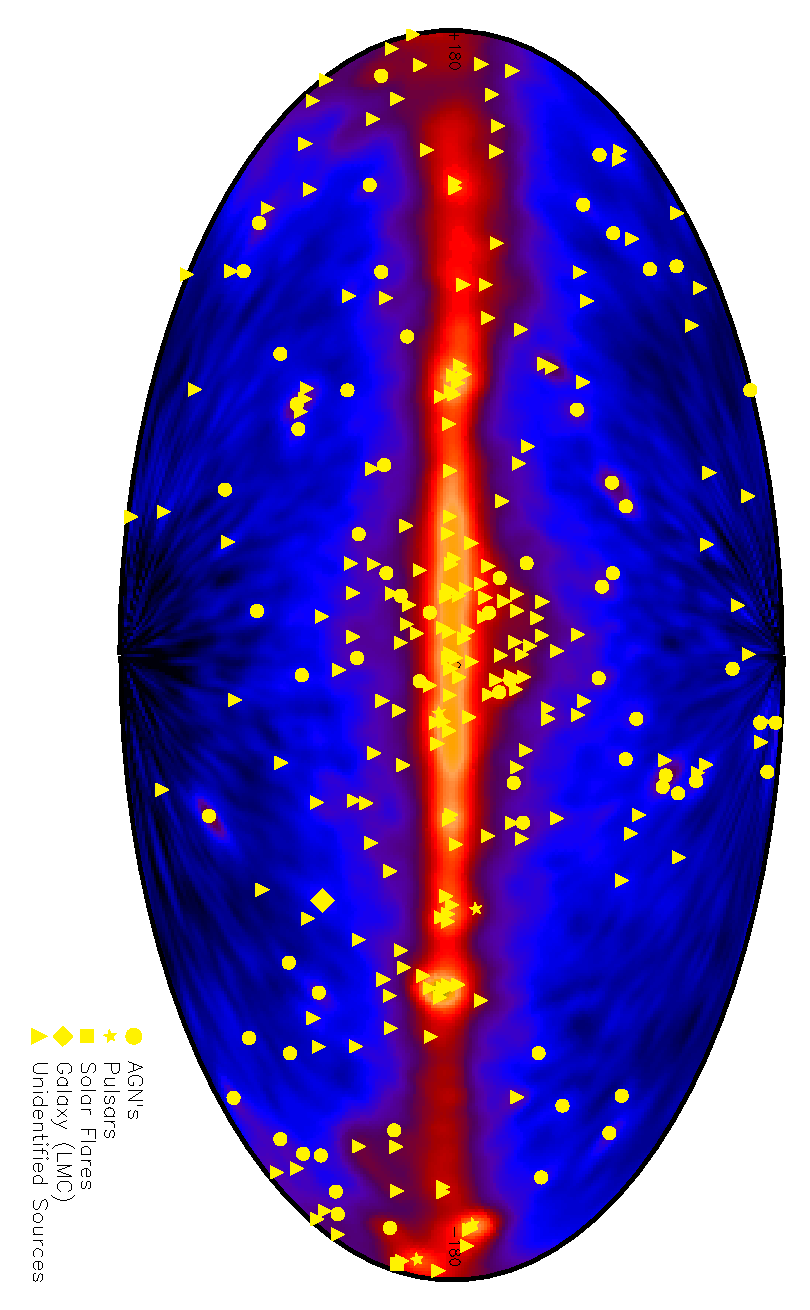
\includegraphics[width=0.8\columnwidth,angle=90]{Figures/3rd_egret_cat.eps} }
	\caption[Third EGRET catalog all-sky map.]{Third EGRET catalog all-sky map. Unidentified sources represented by triangles. Image courtesy of \url{https://heasarc.gsfc.nasa.gov/docs/cgro/images/epo/gallery/skymaps/}}
	\label{fig:3EGSky} 
\end{figure}

 %the predecessor to \FermiLat{} was the \egret{} instrument on \cgro{}. 81 of the 271 \egret{} sources detected were unidentified sources that lied within \blat {} of the Galactic plane.  
 
 Figure \ref{fig:3EGSky} shows an \egret{} all-sky map for ${\rm E > 100 \mev}$ where the preponderance of unidentified sources and locations thereof are made clear. Many studies have tried correlating the unidentified \egret{} sources with various Galactic populations, several of which attempted to assess how likely it was for the low-latitude sources to have an \snr{} origin. The main hindrances to source identification with \egret{} were the numerous potential source counterparts (the instrument's \psf{} was energy dependent, with a 68\% containment radius of ${\rm \sim 6 ^\circ}$ at 100\mev{} and smaller for higher energies) and the large \egret{} error boxes \citep{Hartman99}. For \snrs{} at \gam{} energies, the signature non-thermal \sync{} component that distinguishes radio and X-ray remnants does not typically extend to such high energy, and the other electron and proton loss channels often overlap and are difficult to disentangle (see Chapter \ref{gamAstr:Emiss}). The primary method for identifying a \gam{} source as an \snr{} is through positional coincidence and a compatible angular extent with observations at some other wavelength. Thus the ability to resolve emission from an \snr{} is vital to understanding the mechanisms therein giving rise to \gam{}s.

In spite of the difficulties in \egret{} source association \cite{Sturner95}, \cite{Esposito96}, and \cite{Romero99} found strong evidence for statistical correlation between \snrs{} and some of the low-latitude unidentified sources. In a review of the state of potential \snr{} /  \egret{} associations, \cite{Torres03} showed that there were 19 unidentified \egret{} sources that had an \snr~fall within its 95\% error box. Performing Monte Carlo simulations of the population of  \egret~sources, they determined that the chance probability for the 19 sources to be coincident with an \snr~was $1.05 \times 10^{-5}$, implying a probability of 0.99998 that at least one of the associations was real. Despite the statistical correlation of \egret~sources with \glspl{snr}, there were no definitive associations of an \snr~with any \egret~sources.

As the successor to \egret{}, the \lat{} was designed to improve upon its predecessor in a multitude of areas relevant to detecting \snrs{} \citep{atwood09,lat_perf}. The \lat{} has a much improved angular resolution (68\% single-photon containment radius $\sim 0.4^{\circ}$ at 1\gev{} for photons with the best quality direction reconstruction, PSF3 event type, compared to $\sim 1.7^{\circ}$ for \egret{} at the same energy), which is necessary to resolve \snrs{} as extended objects. The \lat{} also benefits from a superior sensitivity due to a combination of the improved \psf, larger peak effective area ($ {\rm \sim 9500~cm^2}$ vs. ${\rm \sim 1500~cm^2}$), wider \fov{} (2.4 sr, which is nearly 5 times that of \egret{}), and deeper, more-uniform sky exposure (afforded by the \lat's scanning observations as opposed to \egret's pointing operation). All of the above applies to the Pass 8 \irf{} (see Chapter \ref{FGST:LAT} for details on the \lat{}'s performance.

This bump in sensitivity results in the \lat{} detecting considerably more sources than \egret{}. Remarkably, within its first three months of commission, the \lat{} detected 205 sources above {\rm 10$\sigma$ significance \citep{lat_3m}, and by 11 months, 1451 sources above 4$\sigma$ \citep{1FGL}, compared to  the aforementioned 271 over the entire \egret{} mission. In fact, over its lifetime, \egret{} detected a total of about ${\rm 1.5~x~10^6}$ cosmic photons \citep{Thomson93}, while as of June 2016, the \lat{} has detected ${\rm \sim 873~x~10^6}$ events \jamie{this is Source, Clean, UltraClean, UltraCleanVeto events. fair comparison?}. The \lat{}'s point-source sensitivity peaks between 1 and 10\gev{}, depending on location on the sky (see Figures \ref{fig:sensMap} and \ref{fig:sensSlice}). With its increased sensitivity and higher energy range compared to \egret{ }(up to $\sim$ 2\tev{} with the recent Pass 8 event reconstruction improvements, which is nearly an order of magnitude higher than \egret{}), the \lat{} is uniquely situated to study \gam{}s from \snrs{}, with the capability to shed light on \cray{} origins and acceleration mechanisms.
	
Prior to the new work presented in Chapter \ref{chap:snrcat} of this thesis, there had been no systematic study of the population of \lat{} detectable \snrs{}; all reported \lat{} \snrs{} were discovered in individual analyses.  \twofgl{} compiled these results and reported firmly identifying 7 \gam{} sources as \snrs{} and  4 as \pwne{}. 4 2FGL sources were found to be potentially associated with \snrs{} (these were point sources positionally coincident with known \snrs{} but lacking morphological confirmation), and 58 sources were positionally coincident with an \snr{}/ \pwn{} complex, yet it was inconclusive whether the \gam{} emission had an \snr{} or \pwn{} origin. We discuss our contribution (as well as that of others) to the total \lat{} \snr{} population in Chapters \ref{chap:snrcat} and \ref{chap:2FHL}. 

Several classes of \snrs{} have begun emerging from the identified \lat{} \snr{} population. The most numerous of these are Sedov-Taylor phase, evolved \snrs{} (typically composite or mixed-morphology type, and $\gtrsim10^3~ yr$ old). These remnants are typically known to be interacting with nearby molecular clouds through shocked molecular lines, CO line broadening, and possibly OH 1720 MHz maser emission (these systems are sometimes referred to as SNR-MCs). There are two interaction models that exist for accelerating particles to \gam{} emitting energies through interacting with molecular clouds: {\bf 1.}  The ``crushed-clouds" scenario where molecular clouds that have been overtaken by the \snr{} shock  can accelerate \crs{} (or possibly re-accelerate an existing \cray{} population) and produce \gam{}s \citep{Uchiyama10} or {\bf 2.} through the energy dependent escape of high energy \crs{} from the shock of the \snr{} that subsequently diffuse in the surrounding medium and collide with nearby molecular material \cite{Aharonian96,Gabici09,Ohira11}. See Figure \ref{fig:W28} for an example of a \lat{} observed \snr{} with escaping \crs{} interacting with surrounding material. Interactions of these types, \ie{}\ with a dense target material, lead to an observed enhanced luminosity (see Figure \ref{fig:LumDia}, and \ref{fig:LvsD2} for examples of the enhanced luminosity of the \snrs{}) and their emission is often either hadron dominated or shows signs of both leptonic and hadronic emission.

\begin{figure*}[h!]
	\begin{center}
		\hspace*{-2.5cm} 
			\includegraphics[width=1.25\columnwidth]{Figures/{W28cmaps}.png}
	\end{center}
	\caption[\FermiLat{} counts maps from 10-100\gev{} of the region around SNR W28]{\FermiLat{} counts map from 10-100\gev{} of the region around SNR W28. Black circle shows the Green's catalog radius of W28. Left plot shows correlation of the \lat{} emission near W28 with \tev{} illuminated molecular clouds (green contours). Right plot demonstrates\gev{} emission clearly outside the VLA 90 cm image of the shell of W28 (green contours) Figures from \cite{Hanabata14}.
		\label{fig:W28}
	}
\end{figure*}
The second emergent class are the dynamically-young, shell-type \snrs{}. At \lat{} energies these \snrs{} are less luminous, likely due to the shock not expanding for long enough to encounter any surrounding over-density of material. The good correlation between the \gam{} emission and the \snr{} shell suggests that particle acceleration is occurring at the shock front,  and thus the \gam{} rays serve as a direct probe of \dsa{}. These \snrs{} also seem to exhibit harder spectral indices than their evolved counterparts. The hard indices exclude the \dsa{} proton test particle scenario, and are more compatible with an electron test particle \cite{AceroShells}, although this can also be a result of mixed leptonic/hadronic emission, or deviations from the standard hadronic test particle case. 

\begin{figure*}[h!]
	\begin{center}
		%\hspace*{-2.5cm} 
		\includegraphics[width=1.\columnwidth]{Figures/{rxj}.png}
	\end{center}
	\caption[TS map of SNR RX J1713.7-39.46]{TS map for RX J1713.7-39.46 (see Chapter \ref{G150:LATmorph} for definition of TS map) as an example of a \lat{} observed, dynamically young, shell-type \snr{}. Good correlation is shown with the HESS significance contours, shown in white.  Figure from \cite{Federici15}.
		\label{fig:rxj}
	}
\end{figure*}
%Finally there are  a handful of \snrs{} that seem to be at an intermediate stage between the dynamically young and 

The advent of the \lat{} presents for the first time the capability to spectrally and spatially resolve \snrs{} at\gev{} energies, which is important because SNR spectra at \gev{} energies are not just featureless \pl{}s. An unexpected discovery in detecting and studying \snrs{} with the \lat{} is that evolved \snrs{} exhibit a spectral break between 1-10\gev{} \citep{Hewitt15}. Explanations for the break range from Alfv\' en wave evanescence generated by collisions of partially ionized material in \mcs{} overtaken by \snr{}  shocks \citep{Malkov11}, reflected shocks in clouds \cite{Inoue10c}, and energy-dependent diffusion from shocks \cite{Ohira11}. 

In addition to detecting many \snrs{} at \gam{} energies, the \lat{} has been instrumental in providing the first unequivocal evidence of proton acceleration at an \snr{} shock-front. \cite{W44pion} reported observations of  \snrs{} W44 and IC443, which are the two highest flux \snrs{} detected by \lat{} and among the brightest \lat{} sources on the sky. With 4 years of data, and the recent (at the time) Pass 7 updated event-class analysis, \cite{W44pion}, were able to extend the observation energy down to 60\mev{}, significantly detecting the characteristic ``pion-bump" feature (see Chapter \ref{gamAstr:PP} for a description of hadronic \gam{} emission). Detection of this feature by the \lat{} was integral in constraining the \sed{} and hence non-thermal spectral models of each of the \snrs{}. The constrained models demonstrated that a hadronic origin for the observed emission, in both \snrs{}, was the only viable emission mechanism, and that protons can definitively be accelerated by \snr{} shocks.

\begin{figure*}[h!]
	\begin{center}
		%\hspace*{-1.5cm} 
		\begin{tabular}{ll}
			\includegraphics[width=1.0\columnwidth]{Figures/{w44Bump}.png} \\
			\includegraphics[width=1.0\columnwidth]{Figures/{ic443Bump}.png} \\
		\end{tabular}
	\end{center}
	\caption[\gam{} SEDs of SNRs W44 and IC443 obtained with the LAT]{\gam{} \seds{} of \snrs{} W44 (top) and IC443 (bottom) obtained by the \lat{}. Solid lines are for the best-fit pion-decay model, and dashed lines represent the best-fit bremsstrahlung model. A \brems{} model can not sufficiently explain the observed \gam{} emission, unless an ad hoc, low-energy spectral break is included in the \brems{} model (dash-dotted line). Figures from \cite{W44pion}.
		\label{fig:pionBump}
	}
\end{figure*}
%While of key importance in understanding the origin of \crs{} detection of the pion bump in two \snrs{} is not enough, more to do, SNR cat!

%by studying the \gam{} morphology and spectra of \snrs{}. 
	
%Both energetic lepton interactions (\ie{}\ \ic{} radiation of relativistic electrons interacting with ambient photon fields, and non-thermal \brems{}) and hadronic processes ($\pi_0$ decay \gam{}s from \cray{} protons encountering surrounding nuclei) produce spectra observable at \gam{} energies (see Chapter \ref{chap:gamAstr} for details). While the \ic{} generating electron population is also observable through emission of radio \sync{} photons, the proton-proton interaction solely emits \gam{}s.  





\jamie{maybe end with the following to lead into the SNR cat and the rest of the work I do above 1 Gev?}

\jamie{how does this fit in? move to diffuse section?}

Despite being the prime energy range to observe the effects of cosmic particle acceleration, complexities at the lower \lat{} energy range stymie \snr{} morphology studies. The \lat{} detects a strong, soft band of diffuse emission in the Galactic plane due to the interactions of \crs{} with interstellar material. This bright diffuse radiation combined with the multiple potential emission scenarios, broadening \psf{} at decreasing energy, and a high source density in the plane can make it difficult to spatially disentangle sources observed by the \lat{}. To circumvent these 
difficulties, the majority of the analyses undertaken in this thesis are focused on the ${\rm E \geq 1\gev}$ energy range. This energy band is ideal for probing the properties of the accelerated particle populations present in the \snr{} environment. Studies of  \snrs{}  above 1\gev{} benefit from the finer \lat{} \psf{}, striking a balance between minimizing the diffuse contribution, maximizing photon sensitivity, and retaining good photon statistics.

%\section{Summary}\label{Rems:summ} In this section we summarized the end phase of stellar evolution (just enough to motivate SNRs) and descried the environs surrounding the supernova; development and phases of \snrs{}.  In particular we detailed the non-thermal emission mechanisms that produce \g-ray radiation, detection of young vs middle-aged( evolved, interacting with surroundings/dense medium),TeV detects younger typically, the troubles of detecting extension from them(?) something about different emission zones? Troubles disentangling hadronic from leptonic at \g-rays. \g-ray spectral and morphological features. Trends across the population wrt spectral shape/breaks, higher luminosity for interacting rems. Cosmic rays, using gamma-rays to probe CR population. So much of \g-ray astro is really about studying CRs, how much to say about them? 

